\documentclass[12, A4]{report}
\usepackage[ngerman]{babel}
\usepackage[T1]{fontenc}
\usepackage[utf8]{inputenc}
\usepackage{hyperref}
\usepackage{graphicx}
\usepackage{lmodern}
\usepackage[export]{adjustbox}
\usepackage{pdflscape}
\usepackage{helvet}
\usepackage{multirow}
\usepackage[hyperref]{xcolor}

\date{\today}

\begin{document}


\begin{titlepage} %Titelseite
\centering

	{\scshape\LARGE Self Service Terminal for Health Insurance Offices\par}
	\vspace{2cm}

	{\huge\bfseries Review Dokumente\par}
	\vspace{4.5cm}
	{\Large\itshape Jan Angerer, David Hruschka, Yusuf Nowati \par}
	\vspace{0.5cm}
	{\Large\itshape Ziqi Lin, Hakeem Shaddoud, Ahmed Ramadan \par}
	\vfill


	\vfill

% Unterer Seitenabschnitt
	{\large \today\par}
\end{titlepage} %Ende Titelseite


\input{Abkürzungen}
\newpage

\newpage
\tableofcontents  %erzeugt Inhaltsverzeichnis anhand von Chapter und Subsection
\newpage


\chapter{Erstes Review}
\section{Vorgehen}
\subsection{Vorgehensmodell}
Wir haben uns nach Absprache mit unserem Betreuer Professor Matthias Hirth für ein agiles Vorgehensmodell entschieden. Durch den engen Kontakt zu den Auftraggebern ist davon auszugehen, dass sich während der Entwicklung der Software Änderungen an den anfänglich vorgegebnen Anforderungen ergeben. Um möglichst viel Flexibilität zu gewährleisten, bietet sich eine durch Prototypen getriebene Entwicklung an. Die weitergehenden Anforderungen werden im Laufe des Projekts in den Gesprächen mit den Auftraggebern entwickelt. Als Vorgehensmodell orientieren wir uns an einer auf Agilität angepassten Version des Unified Prozess, wie in Abbildung \ref{fig:UPAgil} dargestellt. Dieses Vorgehen harmoniert gut mit der Aufteilung des Softwareprojekts in Phasen, da in 3 Iterationen entwickelt wird.

\begin{figure}[htp]
    \centering
    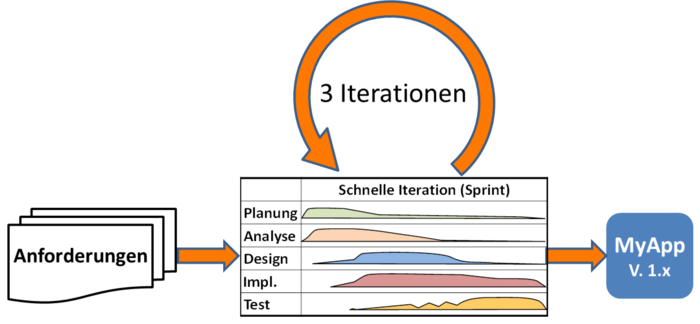
\includegraphics[width=10cm , height=5cm]{Kapitel/Bilder/AgileUnifiedProcess.png}
    \caption[Schema des Vorgehensmodells]{Schema des Vorgehensmodells\protect\footnotemark}
    \label{fig:UPAgil}
\end{figure}
\footnotetext{https://www.tu-ilmenau.de/sse/lehre/softwareprojekt/projektablauf/\#jfmulticontent\_c196637-3, abgerufen am 12.05.2020}

\newpage

\subsection{Alternativen}
\noindent Scrum sowie ExtremeProgramming erscheinen aufgrund der begrenzten Erfahrung des Teams nicht geeignet. Außerdem kann, um das volle Potenzial dieser Verfahren auszuschöpfen, nicht ausreichend Wochenarbeitszeit investiert werden.

\vspace{1,5cm}

\subsection{Durchführung}
\noindent Um einen entwicklungsgetriebenen Ablauf zu gewährleisten arbeiten wir die Projektphasen stark überlappend ab. Vor allem die Phasen "`Analyse"', "`Design"' und "`Implementierung"' werden bei der Entwicklung des Prototypen gleichzeitig ausgeführt. Die entwickelten Anforderungen werden inkrementell implementiert. Aus den gemachten Erfahrungen ergeben sich teils sofort, teils für die weitere Entwicklung, Änderungen. Nach der Implementierung einer Anforderung werden sie in ersten Tests auf ihre Funktionalität überprüft und entsprechende Fehler sofort behoben.

\noindent Ziel der ersten Iteration ist es einen Überblick über Aufwand, Technologie und Risiken zu gewinnen sowie einen lauffähigen Prototypen zu entwickeln. Die Planung der zweiten Iteration basiert auf den Erfahrungen mit dem ersten Prototypen und beginnt nach Präsentation der Ergebnisse der ersten Iteration.

\newpage

\subsection{Werte und Prinzipien}
\vspace{1cm}
\subsubsection*{Werte}

\begin{itemize}
    \item Wir sind als Mitglieder gleichberechtigt und verpflichtet zur Mitarbeit am Projekt.
    \item Wir bringen uns gegenseitigen Respekt und Wertschätzung entgegen.
    \item Wir leben eine offene Kommunikation und Fehlerkultur.
    \item Wir bieten uns gegenseitige Hilfe und Unterstützung an.
\end{itemize}{}

\subsubsection*{Prinzipien}
\begin{itemize}
    \item KISS
    \item Wir halten den Code ständig lauffähig.
    \item Wir arbeiten gemeinsam im Pair-Programming.
    \item Wir machen keine Überstunden.
\end{itemize}{}
      % Einbindung der einzelnen .tex Files
\newpage
\section{Organisation}
Gruppentreffen finden regelmäßig am Donnerstag statt. Die Uhrzeit wird daran angepasst, wann alle Zeit haben. Wir kommunizieren hauptsächlich über das zur Verfügung gestellte RocketChat und über Videokonferenzsysteme. Zum Austausch von Dateien nutzen wir die Nextcloud-Instanz der TU Ilmenau. \\

\noindent Wir haben uns in unserem ersten gemeinsamen Treffen auf eine flache Hierarchie für unser Projekt geeinigt. Gemäß unserer Werte  gilt: Jeder in der Gruppe darf und soll gleichberechtigt an allen Aufgaben mitarbeiten. Trotzdem hat jeder von uns bereits unterschiedliche Kenntnisse und Erfahrungen im Umgang mit den Entwicklungswerkzeugen. Deshalb haben wir zusätzlich folgendes vereinbart:

\noindent Es gibt eine unverbindliche Rollenverteilung auf sogenannte Verantwortliche. Die Verantwortlichen haben ein besonderes Interesse an ihrem Zuteilungsbereich gezeigt, organisieren die gemeinsame Arbeit und sind Ansprechpartner für alle anderen, wenn es Fragen gibt. Sie sind letztendlich dafür verantwortlich, dass ihr Bereich des Projekts erfolgreich ist.\\

\subsubsection*{Momentan gibt es folgende Verantwortliche:}
\begin{itemize}
    \item GitLab: Hakeem Shaddoud
    \item Frontend: Ahmed Ramadan
    \item Dokumentation: David Hruschka und Yusuf Nowati
    \item Modellierung: Ziqi Lin und  Jan Angerer
    \item Projektplanung: Jan Angerer
    \item Backend: David Hruschka
    \item Kommunikation mit Auftraggebern: Jan Angerer
\end{itemize}{}
\vspace{0,5cm}
\noindent Die Zuweisungen können sich im Verlauf des Projekts noch ändern, falls dies von der Gruppe einvernehmlich beschlossen wird.
\newpage
\section{Anforderungsanalyse}
\vspace{0,5cm}

Die gefundenen Anforderungen basieren auf den Inhalten des Lastenhefts, sowie der ersten Besprechung mit den Auftraggebern.


\subsection{Benutzerfunktionen}

\begin{itemize}
    \item \textbf{/F0010/}\textit{Formulare auswählen:} \par
    Ein Benutzer kann Formulare in den Menüs suchen und sich ein Formular anzeigen lassen.
    \item \textbf{/F0020/}\textit{Formulare ausdrucken:} \par
    Ein Benutzer kann ein gefundenes Formular über eine Schaltfläche in der Anwendung ausdrucken.
\end{itemize}
\vspace{1,5cm}
\textbf{Optional:}
    \begin{itemize}
        \item \textbf{/F0030/}\textit{Schnellsuche:} \par
        Der Benutzer kann durch Eingeben eines Suchbegriffs in eine Suchleiste den in der Datenbank hinterlegten Namen eines Formulars direkt suchen. Ist der Name hinterlegt, wird das entsprechende Formular zur Auswahl angezeigt.
        \item \textbf{/F0040/}\textit{eGK einlesen und Formulare vorausfüllen:} \par
        Wurde vom Benutzer ein Formular ausgewählt, kann er seine eGK an einem am IPad angeschlossenen Kartenlesegerät einlesen lassen. Das System füllt das ausgewählte Formular mit den ausgelesenen Daten des Benutzers.
        \item \textbf{/F0050/}\textit{persönliche Beratung durch Videoanruf:} \par
        Der Kunde kann an beliebiger Stelle des Prozesses durch einen Tastendruck einen Videoanruf mit einem Mitarbeiter der Filiale starten.
    \end{itemize}
    
\newpage

\subsection{Administratorfunktionen}

    \begin{itemize}
        \item \textbf{/F0110/}\textit{Einfügen von Formularen:} \par
        Ein Administrator kann Formulare im Format PDF in das Backend hochladen und speichern.
        
        \item \textbf{/F0120/}\textit{Bearbeiten von Formularen:} \par
        Ein Administrator kann die Metadaten eines hochgeladenen und gespeicherten Formulars, wie Titel oder Position in der Menüstruktur, direkt im Backend bearbeiten.
        
        \item \textbf{/F0130/}\textit{Löschen von Formularen:} \par
        Ein Administrator kann ein im Backend gespeichertes Formular aus dem Backend löschen.
        
        \item \textbf{/F0140/}\textit{Setzen der Farben und Logos:} \par 
        Ein Administrator kann die Farben des Frontends anpassen. Außerdem kann er Logos im jpg-Format hochladen und im Frontend anzeigen lassen.
        
        \item \textbf{/F0150/}\textit{Export und Import:} \par
        Die Einstellungen können als JSON Datei exportiert und importiert werden. Die Formulare werden zusammen mit der JSON-Datei in einer Menüstruktur exportiert.
    \end{itemize}{}
\vspace{1,5cm}
\textbf{Optional:}
    \begin{itemize}
        \item \textbf{/F0160/}\textit{Updates:} \par 
        Ein Administrator kann über eine zeitlich begrenzte Internetverbindung das System updaten.
        
        \item \textbf{/F0170/} \textit{Onlinekonfigurationsabgleich:} \par
        Ein Administrator kann den Abgleich der Einstellungen mit einem zentralen Server der Filiale starten.
    \end{itemize}
    
    \newpage
    
\subsection{Systemübersicht}

In Abbildung \ref{fig:UseCase} werden die Nutzungs- und Administrationsanforderungen des Systems sowie die Systemgrenzen als Use-Case-Diagramm dargestellt um einen übersichtlichen Gesamteindruck zu gewinnen.
\vspace{1cm}

\begin{figure}[htp]
    \centering
    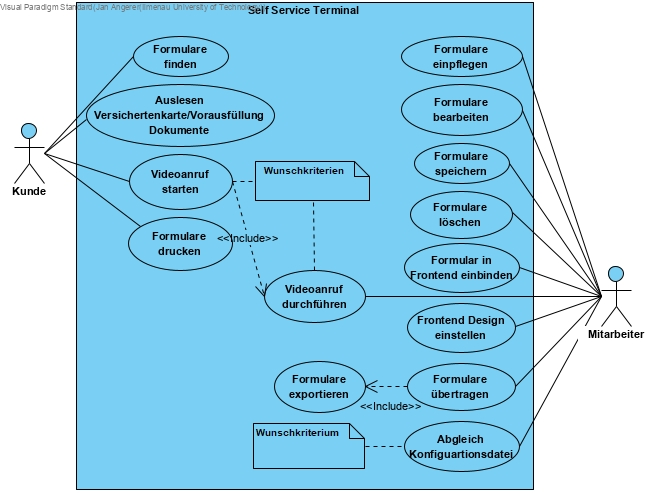
\includegraphics[width=15cm , height=13cm]{Kapitel/Bilder/USeCasev2.jpg}
    \caption{Systemübersicht}
    \label{fig:UseCase}
\end{figure}
\newpage

\subsection{Nicht Funktionale Anforderungen}

\vspace{1cm}

\begin{itemize}
    \item \textbf{/N010/} \textit{Intuitive Bedienbarkeit:} \par
    Die Benutzeroberfläche muss übersichtlich gestaltet werden. Dafür empfehlen sich bildschirmfüllende Schaltflächen mit kontrastreichen Farben. Es sollen nach Möglichkeit nicht mehr als fünf Schaltflächen pro Seite angezeigt werden. 
    
    \item \textbf{/N020/} \textit{Nur eindeutige Eingaben möglich:} \par
    Ein Nutzer soll nur Eingaben tätigen können, die eindeutig sind und genau das ausführen, was sie suggerieren.
    
    \item \textbf{/N030/} \textit{Hohe Performanz:} \par
    Die Reaktionszeit der Benutzeroberfläche beim Klick auf eine Schaltfläche soll dauerhaft unter einer Sekunde liegen.
    
    \item \textbf{/N040/} \textit{Zuverlässigkeit:} \par
    Es soll ein Dauerbetrieb möglich sein. Bei einem Ausfall von Clients soll das System sich automatisch neu starten und wieder lauffähig sein.
    
    \item \textbf{/N050/} \textit{Wartungsarmer Betrieb:} \par
    Einmal eingerichtet soll das System möglichst keine Administratoreingriffe benötigen, bis auf das aktuell Halten der Formulare und Einstellungen. Updates sollen nur in einem Zeitraum $> 3$ Monate nötig sein.
\end{itemize}{}
\newpage
\subsection{Randbedingungen}

\vspace{1cm}
\begin{itemize}
    \item \textbf{/R010/}\textit{Internetzugang:} \par
    Das System darf zum Betrieb keine Internetverbindung benötigen. Dies ist nur während eines Updateprozesses zeitlich begrenzt möglich.
    
    \item \textbf{/R020/}\textit{Betriebssystem:} \par
    Als Betriebssystem ist eine Debian basierte Linux-Distribution vorgegeben.
   
    \item \textbf{/R030/}\textit{Hardware:} \par
    Als Server wird ein \textit{Raspberry Pi} vorgegeben. Als Client fungiert ein \textbf{Apple IPad} mit einer Bildschirmdiagonale von 9 Zoll. Der Ausdruck der Dokumente erfolgt durch einen Netzwerkdrucker oder einen über USB am Server angeschlossenen Drucker.
  
    \item \textbf{/R040/}\textit{Lokales Netzwerk:} \par
    Das System \textit{Raspberry Pi, IPad, Drucker} befinden sich nicht im WLAN der Filiale. Der Pi erzeugt zur Kommunikation ein eigenes Drahtlosnetzwerk.
  
    \item \textbf{/R050/}\textit{Frontend:} \par
    Durch die Nutzung eines \textit{IPads} als Client, muss die Darstellung des Frontends auf dem Safari Browser möglich sein.
  
    \item \textbf{/R060/}\textit{Design:} \par
    Das System soll auch für Menschen Nutzbar sein, welche sich nicht mit Technologie auskennen. Das Nutzerinterface ist daher simpel und deutlich lesbar zu gestalten.
\end{itemize}
\newpage
\section{Entwurfsentscheidungen}
\subsection{Webframework}
Wir haben uns für das Webframework \href{https://www.djangoproject.com/}{Django} entschieden. Gründe dafür sind unter anderem die \href{https://docs.djangoproject.com/en/3.0/faq/general/#faq-mtv}{Abstraktion von Daten und Verhalten im MTV} Prinzip, die bestehende Integration von objektrelationalen Abbildungen für populäre Datenbanksysteme wie MySQL, PostgreSQL oder SQLite. Auch eine automatisch generierte Administratorseite und Djangos Templatesprache zur Generierung von HTML sprachen für Django. Außerdem bietet Django einige Erweiterungen an, die häufige Probleme der Webentwicklung lösen, und es enthält eine sehr ausführliche Dokumentation. \\

\noindent Eine Alternative wäre das in Python geschriebene Webframework Flask. Flask hängt im Gegensatz zu Django nur von der Jinja2 Template Engine und dem WSGI Toolset "`Werkzeug"' ab. Andere Funktionalitäten, wie zum Beispiel objektrelationale Abbildungen, sind nur als Erweiterungen verfügbar.
Flask wurde später als Django veröffentlicht. Deshalb gibt es für Django eine größere Anzahl von Plugins und Erweiterungen. \\

\noindent 
Web2py ist ein freies Webframework für die agile Entwicklung von datenbankbasierten Webanwendungen, welches ebenfalls in Python geschrieben ist. Im Vergleich zu Django hält sich web2py eher an das MVC Prinzip. Es erkennt und rendert Views automatisch. Sein Templatesystem ist keine eigenständige Sprache, sondern besteht aus Pythoncode.
\newpage
\subsection{Programmiersprache}
Zu Beginn des Projektes hatten wir die Wahl zwischen Node.js und Python. Wir haben uns schlussendlich für Python entschieden, da uns die Nutzung des Django Frameworks vielversprechend erschien und Django nur in Verbindung mit Python zu betreiben ist. Der Vorteil in der Nutzung von Node.js hätte in der Asynchronität der IO Operationen gelegen.
\vspace{1,5cm}
\subsection{Datenbank}
Wir haben uns für SQLite als Datenbanksystem entschieden. SQLite weist eine geringe Komplexität und eine geringe Größe auf, eine Datenbank besteht nur aus einer Datei. Unsere Anwendung benötigt nicht viele Schreibzugriffe in kurzer Zeit und es ist auch keine paralleles Schreiben nötig, weshalb SQLite ausreichend ist. SQLite besitzt zudem kein Usermanagement, was aber auch für unsere Anwendung nicht benötigt wird.
\newpage
\section{Grobentwurf}
\subsection {Globaler Kontrollfluss}

Im folgenden Abschnitt erläutern wir den Kontrollfluss der fertigen, initialisierten Anwendung im Einsatz. Eine Visualisierung des Kontrollflusses und der entsprechenden Aktivitäten findet sich in Abbildung \ref{fig:Kontroll}. Wir unterscheiden bei der Bedienung des Systems in zwei Sichten: Mitarbeitersicht und Kundensicht. Die Mitarbeitersicht ist synonym mit Administrator zu verstehen. Wir gehen in dieser Betrachtung davon aus, dass das System im Einsatz und vollständig konfiguriert sowie initialisiert wurde.

\subsubsection{Mitarbeitersicht}
Mitarbeiter oder Administratoren bewegen sich im Backend der Anwendung. Bevor das System durch einen Mitarbeiter der Filiale bedient werden kann, ist es erforderlich sich einzuloggen. Nach erfolgreichem Login können die Mitarbeiter die verfügbaren Aktivitäten in einer Menüstruktur frei wählen. Einzig für die Durchführung der Aktivität nach Kriterium \textbf{/F0170/} ist es notwendig, dass die Anwendung mit einem zentralen Server kommuniziert.

\subsubsection{Kundensicht}
Die Bedienung der Anwendung aus Kundensicht ist deutlich weniger frei als für Mitarbeiter. Um es auch Menschen mit wenig Technikerfahrung zu ermöglichen das System erfolgreich zu bedienen, ist die Anzahl der Wahlmöglichkeiten stark begrenzt.\\
\noindent Formulare werden zuerst in einer Menüstruktur gesucht und danach ausgewählt. Ist ein Formular ausgewählt worden, besteht die Möglichkeit direkt zu drucken, oder die eGK einzulesen um bestimmte Daten in das Formular eintragen zu lassen. Wurde ein Formular gedruckt, springt das System auf die Startseite zurück.\\
\noindent Das starten eines Videoanrufs mit einem Mitarbeiter nach Kriterium \textbf{/F0050/} soll zu jedem Zeitpunkt im Aktivitätsverlauf möglich sein. Ebenso ist es jederzeit möglich, den Prozess abzubrechen und zur Startseite zurückzukehren.

\newpage


\begin{figure}[htp]
    \flushleft
    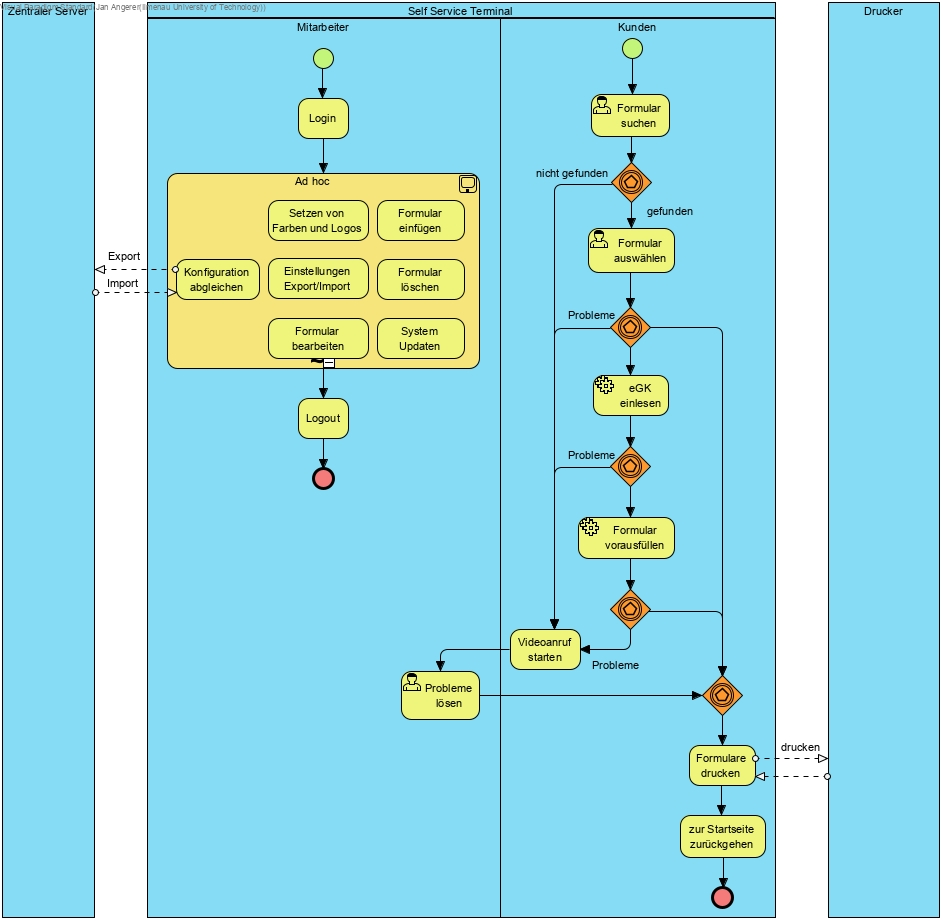
\includegraphics[width=14cm , height=13.5cm]{Kapitel/Bilder/SSTKontrollflussv2.jpg}
    \caption{Kontrollfluss der initialisierten Anwendung}
    \label{fig:Kontroll}
\end{figure}

\newpage
\subsection{Benutzeroberfläche}

\subsubsection{Dialogstruktur}

\textbf{Kundensicht:} \\

\noindent Für die erfolgreiche Bedienung des Systems ist es vor allem wichtig, dass die Kunden möglichst einfach die von ihnen benötigten Formulare finden. Eine Ordnerstruktur erscheint uns zu komplex, weswegen wir auf die Nutzung von Kategorien zurückgreifen. Die Dialogstruktur der Formularsuche ist in Abbildung \ref{fig:DiaglogKunden} beschrieben. Den Kunden werden immer nur die Optionen der horizontalen Ebene angezeigt, auf der sie sich aktuell befinden. Das Ziel ist möglichst wenige Schaltflächen gleichzeitig anzuzeigen. Die abgebildete Struktur orientiert sich an den zur Verfügung stehenden Formularen. Die Anordnung der Schaltflächen erfolgt dynamisch. Es ist also möglich weitere Formulare zu ergänzen. Die Formulierung \textit{Filter} in der Abbildung bezieht sich auf die Filterung der anzuzeigenden Formulare im Backend. \\

\noindent \textbf{Administratorsicht:} \\

\noindent Die konkrete Menüstruktur für die Administratoren sehen wir weniger kritisch als selbige Funktion für die Kunden. Es wird die Fähigkeit vorausgesetzt, sich in einer vordefinierten Menüstruktur zurechtzufinden. Entsprechend ist in Abbildung \ref{fig:DiaglogAdmin} unser Vorschlag für die Implementierung der Menüstruktur im Backend visualisiert. Nach erfolgreichem Login zeigt die Anwendung die Startseite an. Auf der Startseite kann gewählt werden, ob die Einstellungen der Anwendung selbst oder die Formulare gemanagt werden.

\newpage

\thispagestyle{empty}
\begin{landscape}
  \begin{figure}
      \centering
      \includegraphics[scale=0.5, center]{Kapitel/Bilder/Benutzeroberfläche_Kundev2.jpg}
      \caption{Dialogstruktur der Formularsuche aus Kundensicht}
      \label{fig:DiaglogKunden}
  \end{figure}
\end{landscape}

\newpage
\thispagestyle{empty}
\begin{landscape}
  \begin{figure}
      \centering
      \includegraphics[scale=0.6, center]{Kapitel/Bilder/BenutzeroberflächeAdminv2.jpg}
      \caption{Dialogstruktur aus Adminsitratorsicht}
      \label{fig:DiaglogAdmin}
  \end{figure}
\end{landscape}
\newpage

\subsubsection{Bildschirmlayout}

In Abbildung 6 ist ein Beispiel für das fertige Bildschirmlayout zu sehen. Es handelt sich um das Ergebnis eines Medienprojekts an der TU Ilmenau. Zusätzlich zu den gezeigten Schaltflächen, fügen wir einen Button ein, der direkt zurück zum Startbildschirm führt. Die Implementierung einer Schaltfläche zum Starten eines Videoanrufs ist optional.

\begin{figure}[htp]
    \centering
    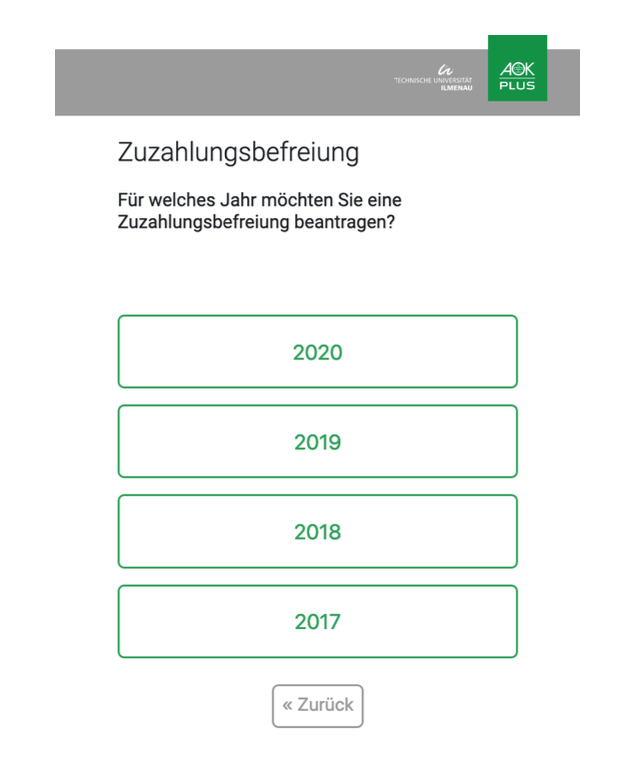
\includegraphics[width=10cm , height=12cm]{Kapitel/Bilder/Interface.png}
    \caption{Benedikt Bieberle, Niclas Deppisch und Robert Schwartz, "`Prototypische Entwicklung eines Self-Service-Terminals für Wartebereiche von Krankenkassenfilianen"', Medienprojekt TU Ilmenau, Mai 2020}
    \label{fig:Interface}
\end{figure}



\newpage




\newpage
\section{Hardware und Software}

Das Self Service Terminal wird auf Debian basierten Betriebssystemen entwickelt und ausschließlich darauf getestet. Zum Betrieb des Systems ist ein Raspberry Pi Einplatinencomputer vorgesehen. Ein solcher Kleinstcomputer eignet sich besonders für den Einsatz als Server für das SST, da er klein gebaut ist und kostengünstig angeschafft werden kann. Als Client wird ein Apple IPad mit einer Bildschirmdiagonale von 9 Zoll eingesetzt, welches hochkant in einem Ständer steht. Der Zugriff auf die Webanwendung erfolgt über den Safari Webbrowser.

\vspace{1,5cm}
\subsection{Software}

\begin{itemize}
  \item Client
    \begin{itemize}
      \item Safari Webbrowser
    \end{itemize}
  \item Server
    \begin{itemize}
      \item Betriebssystem: Raspbian
      \item Python 3 Interpreter
      \item Django Framework
      \item Apache Webserver
      \item SQLite Datenbank
      \item CUPS Druckersoftware
    \end{itemize}
\end{itemize}
\newpage

\subsection{Hardware}


 \begin{itemize}
    \item Client
    \begin{itemize}
      \item 9 Zoll Apple IPad mit Safari Browser
    \end{itemize}
  \item Server
    \begin{itemize}
      \item Raspberry Pi Einplatinencomputer
      \item Netzwerkfähiger Computer zur Administration
      \item Netzwerkfähiger- oder USB-Drucker
    \end{itemize}
\end{itemize}

\vspace{1,5cm}

\subsection{Orgware}

\begin{itemize}
  \item Der Dienst muss einmalig auf dem Raspberry Pi installiert werden und startet nach jedem Neustart von selbst
  \item Gewährleistung einer WLAN Verbindung zwischen Raspberry Pi und IPad
\end{itemize}


\newpage
\section{Persistente Daten}
Das System speichert keine Kundendaten.\par
\vspace{0.5cm}
Folgende Datentypen werden vom System dauerhaft abgelegt:

\begin{itemize}
    \item \textbf{/D010/} \textit{Konfigurationsdatei:} \par
    JSON Datei zur Speicherung des Konfigurationszustands des Systems.
    
    \item \textbf{/D020/} \textit{Formulare:} \par
    Im Backend abgelegte Formulare der AOK im PDF-Format.
    
    \item \textbf{/D030/} \textit{Metadaten:} \par
    .SQLITE Datei mit den Datenbankinhalten zum Betrieb der Anwendung (Views, Models, Templates), sowie Metadaten zu abgelegten Formularen.
    
    \item \textbf{/D040/} \textit{Logos:} \par
    Logos zur Darstellung im Frontend als JPEG Dateien
    
    \item \textbf{/D050/} \textit{Logindaten:} \par
    Verschlüsselte Logindaten des Administrator-Kontos
\end{itemize}
\newpage
\section{Technologien und Entwicklungsumgebung}
\subsection{Frontend}
Das Frontend wird mit HTML, CSS und JavaScript entwickelt. Für die Generierung von Seiten wir die Django Templatesprache verwendet.

\subsection{Backend}
Im Backend läuft ein Apache Webserver und das Django Webframework. Das Framework führt den Pythoncode aus, in dem die Modelle und Views geschrieben sind. Der Kleinstrechner stellt einen WLAN Access Point bereit, zu dem sich die Clients verbinden, um auf die Kunden- und Administratorseiten zuzugreifen.

\subsection{Entwicklungstools}
Als IDE verwenden wir Visual Studio Code. \\
Gitlab dient als Versionsverwaltung, mit dem eingebauten Wiki als Dokumentation und als Bugtracker. Zum Testen werden ein bereitgestelltes iPad, sowie ein Raspberry Pi genutzt. \\
Für das Pflichtenheft und die Reviewdokumente verwenden wir den Online-Latex-Editor Overleaf.
\newpage
\section{Ergebnisse der ersten Iteration}
Neben der Organisation des Teams und der Auswahl der Entwicklungswerkzeuge stellen die Inhalte des Pflichtenhefts die zentralen Ergebnisse der ersten Iteration dar. Die dort definierten funktionalen und nichtfunktionalen Anforderungen bilden die Grundlage für die kommenden Weiterentwicklungen des Prototypen. Aus dieser Grundlage entstand der Entwurf und wurde in Ansätzen bereits implementiert.
\section{Ausblick auf die zweite Iteration}
Das Ziel der zweiten Iteration besteht in der Implementierung aller Musskriterien. Dabei sollen bereits Testfälle definiert und implementiert werden. Optional soll an den Wunschkriterien gearbeitet werden. Hier sollen ebenso Tests implementiert werden. Die Arbeitsweise ist wie folgt: \\

\noindent Alle Anforderungen werden als Issues in Gitlab eingetragen und können einzelnen Teammitgliedern zugewiesen werden. Der aktuelle Stand wird im Kommentarbereich des Issues dokumentiert. Wenn eine Anforderung fertiggestellt und getestet worden ist, wird das Issue geschlossen. Die Anforderungen sind vergleichbar mit den "`user stories"', die in der agilen Entwicklung verwendet werden. Alle zwei Wochen trifft sich die Große Runde bestehend aus allen Teammitgliedern, den Betreuern und Auftraggebern und tauscht sich über den Fortschritt des Projekts aus. Es wird der aktuelle Prototyp vorgeführt. \\

\noindent Am Ende der zweiten Iteration soll als Ergebnis ein Prototyp stehen, der alle Musskriterien erfüllt. Außerdem soll der erstellte Code dokumentiert worden sein. Ein Model-Template-View Diagramm stellt die innere Struktur der Software dar. 
\chapter{Zweites Review}
\section{Feinentwurf}
\subsection{Vorüberlegungen}
Im Zuge der Erstellung des Feinentwurfs wird das Analysemodell des Grobentwurfs in fachlicher Hinsicher vervollständigt. Üblicherweise erfolgt dies durch Definition von Klassen, Attributen, Operationen und Assoziationen in einem Klassendiagramm. Das Self-Service-Terminal wird jedoch als Webapplikation in einem gesetzten Framework entwickelt und muss daher besonderen Anforderungen genügen.
Das Django Framework trennt Datenverarbeitung, Websitedesign und Logik voneinander, damit diese Elemente möglichst unabhängig von einander entwickelt werden können. Aufgrund dessen erscheint es sinnvoll den Feinentwurf nach der Struktur des Model-Template-View-Prinzips zu entwickeln. Struktur und Aufbau der MTV-Architektur sowie die Zusammenhänge der Elemente untereinander werden in \ref{fig:MVT_Erweitert} visualisiert.

\subsection{Model-Template-View-Prinzip}
Das Model-Template-View-Prinzip basiert auf einer möglichst losen Kopplung der Softwareelemente Model, Template und View. Die Aufgaben der entsprechenden Elemente unterscheiden sich dabei naturgemäß voneinander:\par 
\vspace{0,5cm}
\noindent \textbf{Models:} \par
\vspace{0,5cm}
\noindent Durch Models wird die Datenverarbeitung der Webapplikation gesteuert. Grundsätzlich gilt, dass jede Klasse der Models einer Relation in der zugrundeliegenden Datenbank entspricht. Die erstellten Klassen sind dabei Pythen Unterklassen der Klasse \textit{django.db.models.Model}. Die Attribute der generierten Klassen entsprechen dabei den Attributen der jeweiligen Relation. Zusammen ergeben sie also das Relationsschema. Anhand dieser Informationen steuert Django Anfragen an die Datenbank mithilfe der \textit{database-access API} automatisch.\par
\vspace{0,5cm}
\noindent \textbf{Templates:}\par
\vspace{0,5cm}
\noindent Djangos Templates enthalten Informationen über die Ausgabe statischer und dynamischer HTML Elemente. Mithilfe der Django-Templatesprache ist es außerdem möglich Inhalte in Blocks aufzuteilen und diese dynamischen Inhalte aufzurufen. Django nutzt eine eigene Schnittstelle zum laden und rendern der Templates.

\newpage

\noindent \textbf{Views:}\par
\vspace{0,5cm}
\noindent Views sind Funktionen, welche eine http-Request übergeben bekommen und eine http-Response zurückgeben. Das View enthält dabei die dazu notwendige Logik. Um die Projektstruktur möglichst einfach zu halten, legen wir auch andere anwendungsbezogene Logik in der view.py Datei ab. Nur Funktionen, die direkt mit den Model-Klassen interagieren werden in der model.py abgelegt.\par
\vspace{1cm}
\begin{figure}[htp]
    \centering
    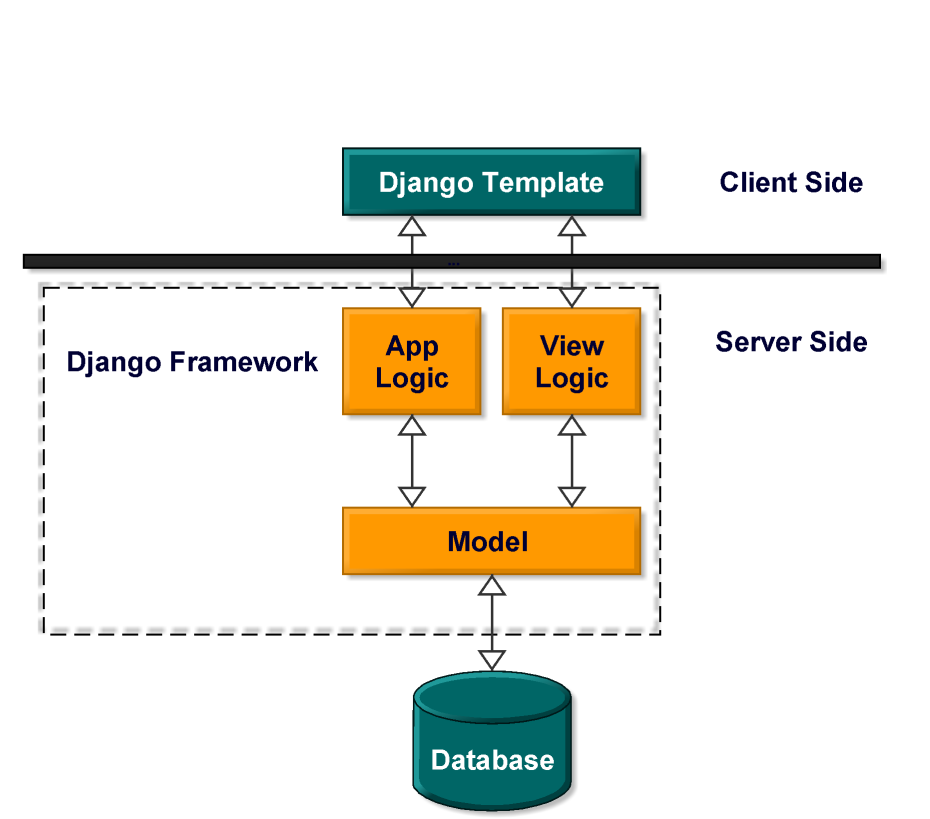
\includegraphics[width=12cm , height=11cm]{Kapitel/Bilder/MVT-Erweitert-Diesmalwirklich.PNG}
    \caption{Visualisierung des MVT-Prinzips im Django Framework}
    \label{fig:MVT_Erweitert}
\end{figure}
\newpage
\subsection{Architektur des Self-Service-Terminal}
Die Entwicklung des SST wird iterativ durchgeführt und orientiert sich an den zu erfüllenden Anforderungen. Die Architektur des Systems entwickelt sich daher im Geiste des gewählten agilen Vorgehensmodells Stück für Stück mit den implementierten Anforderungen. Das MTV-Prinzip gibt dabei die Struktur vor. 


 %Inhalt da 
sd.fkglhjnsydlkfjgnsödofjgnsöodfggbn
\newpage
\input{Kapitel/Problemlösung}
\newpage
\section{Schnittstellendokumentation}
Das Self-Service-Terminal benötigt zum Abschluss der zweiten Iteration an drei Stellen Zugriff auf Schnittstellen. Einmal sind einige Schnittstellen innerhalb der Systemgrenzen notwendig um die Grundfunktionalität des Django Frameworks sicherzustellen. Diese Schnittstellen bringt das Framework mit, sie werden automatisch genutzt, wenn in Django nach dem MTV-Prinzip gearbeitet wird. Darüber hinaus kommuniziert das Selt-Service-Terminal noch mit der CUPS-Druckersoftware und dem Apache Webserver über das Apache Modul: Web Server Gateway Interface (mod\_wsgi).
\subsection{Django}
Innerhalb Systemgrenzen des SST werden ausschließlich die Schnittstellen verwendet, welche Django aufgrund seines Aufbaus mitbringt. Der Verwendung dieser Schnittstellen ergibt sich automatisch, wenn eine Webanwendung nach dem Model-Template-View-Prinzip entwickelt wird. Als Beispiel möchten wir kurz die sogenannten \glqq Manager\grqq{} anführen. Als Manager werden in Django die Schnittstellen bezeichnet, durch welche Datenbank-Anfrage-Operationen für die Modelle realisiert werden. Standardmäßig wird für jedes Modell eine solche Manger-Klasse angelegt. Details zur Verwendung von Schnittstellen im Django Framework lassen sich der Django \footnote{\href{https://docs.djangoproject.com/en/3.0/}{https://docs.djangoproject.com/en/3.0/}}Dokumentation entnehmen.

\subsection{CUPS}
Das Self-Service-Terminal verwendet die CUPS-Druckersoftware um die Druckfunktionalität für ausgewählte Formulare über den Raspberry Pi umzusetzen. Dazu wird ein Python-Subprocess aufgerufen, der die Kommandozeile aufruft. Der Kommandozeile wird der Befehl: lpr \textit{Dateiname} übergeben. Die Rückgabe der Kommandozeile wird als OBjekt zurück an das SST geschickt. Das Objekt enthält die Standard-Datenströme \textit{stderr}, \textit{stdout} und der Rückgabewert des \textit{lpr}-Befehls. Aufgrund dieser Informationen wird der Druckvorgang entweder bestätigt, oder eine Fehlermeldung ausgegeben. 
\subsection{mod\_wsgi}
Um die Kommunikation einer Python-Anwendung mit dem Apache Webserver zu gewährleisten ist es erforderlich Apache um das Modul \textit{mod\_wsgi} zu erweitern. WSGI ist dabei der Standard für Python Webapplikationen. Genauere Informationen zur Funktionsweise des Moduls sind in der \footnote{\href{https://modwsgi.readthedocs.io/en/develop/index.html}{https://modwsgi.readthedocs.io/en/develop/index.html}} zu finden.

\newpage
 \section{Bugreview}
 \subsection{Aufnahme von Bugs}
 Bugs werden vom Self-Service-Terminal Team im Bugtracker des zur Verfügung gestellten GitLabs angelegt. Der Bugtracker ist die zentrale Sammelstelle für alle gefundenen Bugs. Jedes Teammitglied hat Zugriff auf die Funktion und kann sich Bugs zuweisen, um sie anschließend zu bearbeiten. Dieser Vorgang wird manuell durchgeführt. Die entsprechend angelegten Issues werden mit einem eindeutig identifizierbaren Namen versehen. Außerdem kann den Issues ein Fälligkeitsdatum sowie ein korrespondierender Milestone zugewiesen werden. Abhängig von der Stelle an der ein Bug aufgetreten ist, wird er mit zugehörigen Tags versehen. Aktuell wird in den Tags zwischen \glqq Frontend\grqq{} und \glqq Backend\grqq{} unterschieden. Ein Issue kann das \glqq Frontend\grqq{}, \glqq Backend\grqq{} und beide Tags gleichzeitig zugeordnet bekommen.
 \vspace{1cm}
 \subsection{Priorisierung}
 Um gefundene Bugs in einer zielführenden Reihenfolge abzuarbeiten werden diese im Bugtracker durch Tags priorisiert. Die Priorisierung wird in einer Weise durchgeführt, sodass deutlich erkennbar ist wann ein Bug behoben sein muss um die gewünschte Funktionalität der Anwendung zu den gesetzten Deadlines zu erreichen. Die Deadlines werden hierbei durch eine Verknüpfung der Issues mit den Meilensteinen \glqq 2. Review\grqq{} und \glqq Testphase\grqq{} repräsentiert. Es wird außerdem zwischen der Schwere der Bugs unterschieden. Bugs, welche die Anwendung in der Erfüllung der Musskriterien hindert, werden mit dem Tag \glqq critical\grqq{} versehen. Diese Bugs haben gemessen an der zugehörigen Deadline die höchste Priorität.
 \newpage
 \subsection{Liste aufgenommener Bugs}
\begin{itemize}
    \item \textbf{/B001/} | \textcolor{violet}{Frontend} | \textcolor{cyan}{2. Review} | \\ \noindent \textit{\textbf{Unterscheidung von Formularen und Submenus in angezeigten Menus:}} \\ \noindent Formulare und Untermenus innerhalb von Menus lassen sich nur durch den angezeigten Text unterscheiden. Eine grafische Unterscheidungsmöglichkeit ist notwendig.
    \item \textbf{/B002/} | \textcolor{violet}{Backend} | \textcolor{cyan}{Testphase} | \\ \noindent \textit{\textbf{Hilfe Template bei nicht gesetzter Startseite anzeigen:}} \\ \noindent Die Startseite fungiert als Wurzel der Baumstruktur von Menus und Formularen. Ist die Startseite nicht gesetzt, kann die Menüstruktur nicht erzeugt werden. Ist keine Startseite gesetzt, sollte ein Hilfetext angezeigt werden.
    \item \textbf{/B003/} | \textcolor{violet}{Backend} | \textcolor{cyan}{2. Review} | \\ \noindent \textit{\textbf{Usability im Admin-Panel:}} \\ \noindent Wurde im Admin-Menü ein \textit{Terminal\_Settings} ForeignKey festgelegt, soll er für alle weiteren Untermenüs voreingestellt sein.
\end{itemize}
\newpage
\section{Ausblick auf die dritte Iteration}
\subsection{Testen des Systems}
Hauptaufgabe während der dritten Iteration ist das Testen des Self-Service-Terminal. Wir werden dafür automatische Tests definieren, um die implementierten Anforderungen ausführlich zu testen. Gefundene Bugs werden gemäß unserer Problemlösungsverfahren an Teammitglieder deligiert und behoben. Ziel ist es zum Ende der dritten Iteration alle Musskriterien fehlerfrei implementiert zu haben. Die zweite Hauptaufgabe während der Testphase besteht darin, das User-Interface auf Bedienbarkeit zu prüfen und gegebenenfalls Anpassungen vorzunehmen.\par
\vspace{0,5cm}
\subsection{Konfiguration der Hardware}
Das Self-Service-Terminal soll auf einem Raspberry Pi zum Einsatz kommen. Um die Randbedingungen für den Betrieb der Anwendung zu erfüllen, muss der Pi entsprechend konfiguriert werden. Diese Konfiguration soll nach Möglichkeit automatisch erfolgen, wenn die Anwendung installiert wird. Dazu wird ein Installationsskript nötig sein, dass bei der Installation ausgeführt wird. Dieses Skript wird in der 3. Iteration entwickelt und getestet. \par
\vspace{0,5cm}
\subsection{Deployment}
Das Self-Service-Terminal muss zum Abschluss der Entwicklung von der Entwicklungsumgebung in die Produktivumgebung überführt werden. Dazu ist es notwendig, vom Django-Entwicklungsserver auf einen Apache Webserver mit dem \textit{mod\_wsgi} Modul zu wechseln. Es muss außerdem eine Lösung entwickelt werden, das System möglichst benutzerfreundlich aufzusetzen.

\newpage
\chapter{Drittes Review}
\newpage

\section{Glossar}

\begin{description}
  \item[Back-End]
    Nur für Administratoren zugängliche Seiten zur Systemverwaltung, d.h. Einpflegen, Speichern, Bearbeiten, Exportieren und Löschen von Formularen sowie das Einstellen von Farbschemata und Logos im Front-End.
 
  \item[Django]
    ist ein in Python geschriebenes, quelloffenes Webframework, das einem Model-Template-View-Schema folgt.
    \footnote{\href{https://docs.djangoproject.com/en/dev/faq/general}{docs.djangoproject.com/en/dev/faq/general, abgerufen am 08.05.2020}}

 \item[Elektronische Gesundheitskarte]
    Chipkarte im Scheckkartenformat, die als erweiterte Versichertenkarte für gesetzlich Krankenversicherte fungiert.
    \footnote{\href{https://de.wikipedia.org/w/index.php?title=Elektronische_Gesundheitskarte&oldid=198562236}{de.wikipedia.org/w/index.php?title=Elektronische\_Gesundheitskarte,  abgerufen am 08.05.2020}}
    \footnote{\href{https://www.gesetze-im-internet.de/sgb_5/__291.html}{www.gesetze-im-internet.de/sgb\_5/\_\_291.html, abgerufen am 08.05.2020}}
 
  \item[Front-End]
    Webseite für die Kundenoberfläche.
    
  \item[Git]
    ist eine freie Software zur verteilten Versionsverwaltung von Dateien.
    \footnote{\href{https://de.wikipedia.org/w/index.php?title=Git&oldid=199354247}{de.wikipedia.org/w/index.php?title=Git, abgerufen am 09.05.2020}}
    
  \item[GitLab]
    ist eine Webanwendung zur Versionsverwaltung für Softwareprojekte auf Basis von Git.
    \footnote{\href{https://de.wikipedia.org/w/index.php?title=GitLab&oldid=196028257}{de.wikipedia.org/w/index.php?title=GitLab, abgerufen am 09.05.2020}}
    
  \item[KISS]
    "Keep it small and simple" bzw "Keep it simple, stupid". Ist ein Prinzip der agilen Vorgehensweise welches besagt, dass zu einem Problem eine möglichst einfache Lösung gefunden werden soll.

  \item[iPad]
    Tabletcomputer des Herstellers Apple Inc.

  \item[Model Layer]
    Eine Abstraktionsschicht in Django, die zur Strukturierung und Manipulation der Daten der Webapplikation dient.
    \footnote{\href{https://docs.djangoproject.com/en/3.0/}{docs.djangoproject.com/en/3.0/, abgerufen am 08.05.2020}}
 
  \item[Model-Template-View]
    Djangos Umsetzung des Model-View-Controller Musters.

  \item[Model-View-Controller]
    Model View Controller ist ein Muster zur Unterteilung einer Software in die drei Komponenten: Datenmodell (model), Präsentation (view) und Programmsteuerung (controller).
    \footnote{\href{https://de.wikipedia.org/w/index.php?title=Model_View_Controller&oldid=195305891}{de.wikipedia.org/w/index.php?title=Model\_View\_Controller, abgerufen am 08.05.2020}}
    
  \item[Overleaf]    
    ist ein Online LaTeX Editor. 

  \item[Python]
    ist eine universelle, interpretierte, multiparadigmatische Programmiersprache.
 
  \item[Views]
    Kapseln in Django die Logik, welche für die Verarbeitung der Anfrage eines Nutzer und die Rückgabe einer Antwort verantwortlich ist.

  \item[Raspbian]
    Linux-Betriebssystem auf Basis von Debian. Wird hauptsächlich auf den Raspberry Pi Einplatinencomputern eingesetzt.
    
  \item[RocketChat]
    ist eine freie und quelloffene Chatsoftware.

  \item[Self-Service-Terminal]
    Ein Computer, der von Kunden in einem Geschäft oder einer anderen Einrichtung zur Selbstbedienung genutzt werden kann. Oftmals mit eingebautem Touchscreen.
\end{description}


\end{document}
